% reviewers: Zam, Jared, Heng Li, Mike Schatz?, lighter
% @funding acks, torng, charles, sebastian.

\documentclass{article}
\usepackage{graphicx}
\bibliographystyle{plos2009}

\usepackage{lineno}
\linenumbers

\begin{document}

\title{Crossing the streams: a framework for semi-streaming analysis of
short DNA sequencing reads}

\author{Qingpeng Zhang$^{1}$, Sherine Awad$^{2,3}$, C. Titus Brown$^{2,1,3,\ast}$\\
\small
\bf{1} Computer Science and Engineering,\\
\small
Michigan State University,
East Lansing, MI, USA
\\
\small
\bf{2} Microbiology and Molecular Genetics,\\
\small
Michigan State University,
East Lansing, MI, USA
\\
\small
\bf{3} Population Health and Reproduction,\\
\small
University of California, Davis, Davis, CA, USA
\\
\small
$\ast$ E-mail: ctbrown@ucdavis.edu
}
\maketitle


\abstract{We present a semi-streaming algorithm for k-mer spectral
  analysis of DNA sequencing reads, together with a derivative
  approach that is fully streaming.  The approach can also be applied
  to genomic, transcriptomic, and metagenomic data sets.  We develop
  two tools for short-read analysis based on these approaches, a
  method for semi-streaming k-mer-based error trimming, and a method
  for the analysis of error profiles in short reads using a streaming
  sublinear approach. These tools are implemented in the khmer
  software package, which is freely available under the BSD License at
  github.com/ged-lab/khmer/.}

\section{Introduction}

K-mer spectral analysis is a powerful approach to error detection and
correction in shotgun sequencing data that uses k-mer abundances to
find likely errors in the data \cite{Pevzner2001}.  Approaches derived
from spectral analysis can be very effective: spectral error
correction achieves high accuracy, and Zhang et al. (2014) show that
spectral k-mer trimming is considerably more effective at removing
errors than quality score-based approaches
\cite{quake,Zhang2014}.  However, spectral analysis is also very
compute intensive: most implementations count all the k-mers in
sequencing data sets, which can be memory- or I/O-intensive for large
data sets \cite{Zhang2014}.

Streaming and semi-streaming algorithms can offer improved algorithmic
and computational efficiency in the analysis of large data sets
\cite{Charikar2004, Cormode2005}.  Streaming algorithms typically
examine the data only once, and have small, fixed memory usage.
Semi-streaming algorithms may examine the data a few times, with
memory requirements that scale sublinearly with the size of the input
data \cite{Feigenbaum2005}.  Streaming algorithms have not been
applied to k-mer spectral analysis of sequencing reads, although
Melsted et al. developed an effective streaming algorithm for
calculating {\em aggregate} statistics of k-mer distributions from
sequencing data \cite{Melsted2014}, and the Lighter error corrector
uses a low-memory semi-streaming multipass approach to do efficient
error correction \cite{lighter}.
% mention express? No, not really k-mers.

Brown et al. (2012) introduced a streaming algorithm for downsampling
read data sets to normalize read coverage spectra, termed ``digital
normalization'' (or ``diginorm'') \cite{Brown2012}.  This procedure
estimates the k-mer coverage of each read in a stream using an online
algorithm. Reads above a certain estimated coverage are set aside and
their k-mers are not tracked.  The diginorm algorithm only examines
the data once, and counts only the k-mers in retained reads, leading
to sublinear memory usage for high-coverage data sets
\cite{Brown2012}.

While the abundance normalization process developed in digital
normalization has been used widely (\cite{xxx}) and is now implemented
in several different software packages \cite{yyy}, the streaming
approach itself has not been developed further.  Here we develop a
semi-streaming algorithm for k-mer spectral analysis, based on digital
normalization, that can detect and remove errors in sequencing reads.
This algorithm operates in sublinear memory with respect to the input
data, and examines the data at most twice.  The approach offers a
general framework for streaming sequence analysis and could be used
for error correction and variant calling.  Moreover, the approach can
be applied generically to data sets with variable sequencing coverage
such as transcriptomes, metagenomes, and amplified genomic DNA.  We
also provide a fully streaming approach for estimating per-position
sequencing error rates in reads that operates in fixed memory and only
examines part of the input data.

\subsection{Algorithmic considerations}

\label{sec:alg}

Shotgun DNA sequencing gives us a stream
of items representing sentences (``reads'') randomly sampled from a
larger text, with replacement.  In this paper, our primary goal is to
efficiently identify the locations of errors in these reads by
finding differences with respect to the (unknown) source text; however, this
problem is a gateway to a larger set of interesting domain problems,
which includes estimating the true abundance of the sentences in the
larger text and determining the complete composition of the source text.

There are several distinct features of this problem that bear
mentioning.  The first is that important details of the source text,
such as its size and statistical composition, may be completely
unknown; that is, often the reads themselves are the most specific
information we have about the source text.  Second, the source text
may be incompletely sampled by the reads, and whether or not it is
completely sampled may not be known in advance.  And third, read
data sets are typically stored on disk, at least in current
implementations; our goal is to identify more efficient approaches to
examining these data sets without necessarily moving to a pure
streaming model, which allows us to make use of the {\em
  semi-streaming} paradigm introduced by Feigenbaum et
al. \cite{Feigenbaum2005}.

We address this problem by making use of k-mer spectra, a common
approach in which reads are treated as subpaths through a De Bruijn
graph, and errors in the reads are identified by finding low-frequency
subpaths \cite{Pevzner2001}.  Below, we generalize this approach by
building the graph with an online algorithm and detecting regions of
the graph saturated by observations.  These regions can then be used
for per-read analysis without necessarily examining the entire data
set.

\paragraph{Detecting graph saturation:}
We detect graph saturation with digital normalization, presented
in \cite{Brown2012}. The digital
normalization algorithm is, in Python pseudocode:
\begin{verbatim}
for read in data:
   if coverage(read, table) < DESIRED:
      add_read_to_graph(read, graph)
      analyze(read)
\end{verbatim}
This is a single-pass algorithm that can be implemented in fixed space
using a Count-Min Sketch to store the De Bruijn graph necessary for
coverage estimation \cite{Pell2012, Zhang2014}.  For any
error-containing data set with coverage greater than {\tt DESIRED},
the graph requires space less than the size of the input - typically
space sublinear in the data size, for any fixed-size source text (see
Figure~\ref{fig:saturation} and \cite{Zhang2014}).

\begin{figure}[!ht]
 \centerline{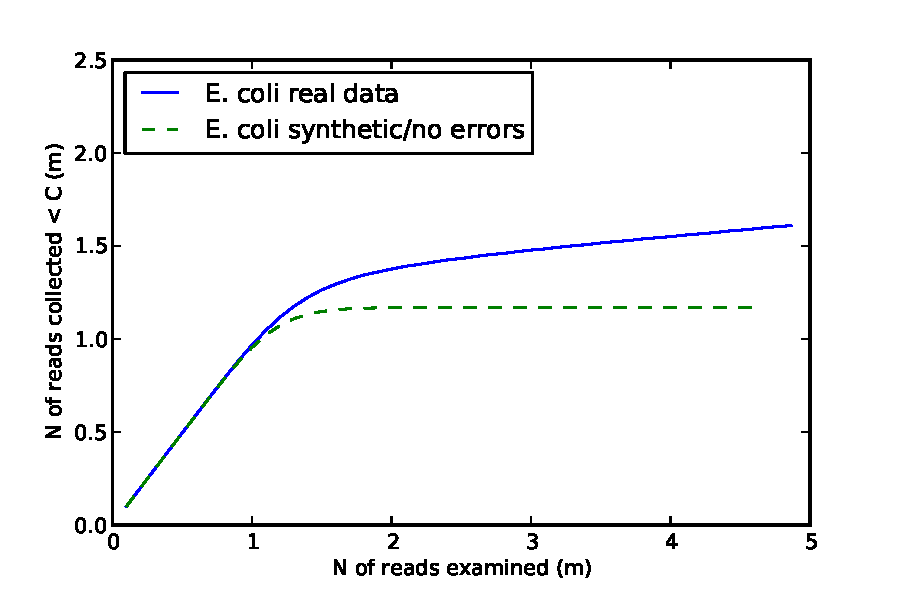
\includegraphics[width=4in]{./figures/saturation}}
\caption{\bf Saturation curve of a real and a simulated {\em E. coli}
  read data set.  Reads are collected when they have an estimated
  coverage of less than 20; in the early phase ($<$ 1m reads), almost
  all reads are collected, but by 2m reads into the data set, the
  majority of reads come from loci with an estimated sequencing depth
  of $>$ 20 and are rejected.}
\label{fig:saturation}
\end{figure}

The digital normalization algorithm was developed as a {\em filter},
in which retained reads are passed on to another program (such as a {\em
  de novo} assembler) for further analysis -- these later analyses are
typically based on multi-pass, heavyweight algorithms.  Here, digital
normalization is performing lossy compression, reducing the number of
error-containing sentences while attempting to retain the structure of
the De Bruijn graph \cite{Brown2012, Zhang2014, Lowe2015}.  This reliance
on a post-normalization heavyweight analysis step presents challenges in the
analysis of large data sets, which motivates this work.

\paragraph{Semi-streaming analysis:} The algorithm for {\em semi-streaming} analysis of reads we explore in this work is:
\begin{verbatim}
for read in data:  # first pass
   if coverage(read, graph) < DESIRED:
      add_read_to_graph(read, graph)
      save(read)
   else:
      analyze(read)

for read in saved_reads:   # second pass
   if coverage(read, graph) >= DESIRED:
      analyze(read)
\end{verbatim}
Here, the space used for the graph remains identical to the digital
normalization algorithm and is typically sublinear in space for high
coverage data sets, but the algorithm is no longer single-pass, and
requires re-examining some subset of the input data in a second pass.
In the worst case scenario, with an undersampled source text (or
randomly generated sentences), this is a fully offline two-pass
approach that requires re-examining {\em all} of the input data for
the second pass.  In practice, most real data sets will require fewer
than two passes: graphically, any deviation from the identity line in
a saturation analysis as in Figure~\ref{fig:saturation} yields a
few-pass algorithm.

\paragraph{Reduction to a streaming algorithm:} The semi-streaming
algorithm can be turned into a purely streaming algorithm in several
special cases - specifically, whenever reads need not be saved for a
second pass.  One example is given below, in determining the error
profile of sequencing reads: here the error profile can be determined
from only a small portion of the data.

Another example of a purely streaming approach is when some portion of
correct data can be discarded, e.g. because of oversampling.  (One
biological application for this occurs when the data set generated is
large enough to guarantee very high coverage of the entire genome.)
In this case, rather than saving reads for a second pass, only
saturated reads are analyzed, while reads that are not from saturated
regions in the graph are simply discarded.  Applying this approach to
the {\em E. coli} data set used above for Figure~\ref{fig:saturation},
approximately 1/3 of the reads would be discarded while the remaining
2/3 would be analyzed (see ``Number of passes'',
Table~\ref{tab:spectra_streaming_real}).

\begin{figure}[!ht]
 \centerline{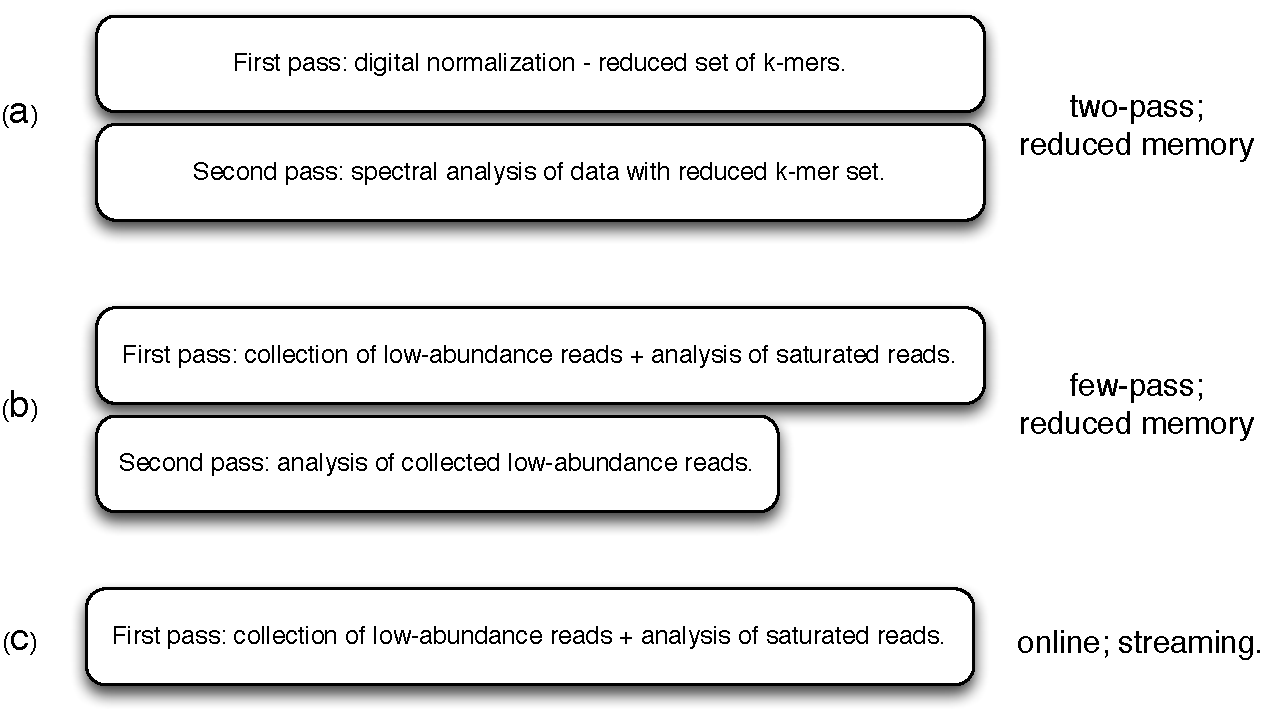
\includegraphics[width=4in]{./figures/summary-algorithms}}
\caption{\bf A summary of the three approaches to k-mer spectral analysis
  presented below.  (a) Digital normalization reduces the set of k-mers
  to be used for the second pass analysis of the full data set. (b) Combining
  online saturation analysis with collection of reads yields a few-pass
  algorithm.  (c) When all of the data does not need to be analyzed, online
  detection of saturation can be used to drive the analysis of saturated
  portions of the reads and graph.}
\label{fig:summary}
\end{figure}

\paragraph{Summary:} A summary of the three approaches described above
is presented in Figure~\ref{fig:summary}.  The two-pass approach in
Figure~\ref{fig:summary}(a) yields more efficient memory use, but with
no advantage in execution time.  The few-pass approach
(Figure~\ref{fig:summary}(b)) combines the lower memory use with fewer
passes across the data, and becomes more efficient as the coverage of
the data set grows.  Finally, the fully streaming approach in
Figure~\ref{fig:summary}(c) enables one-pass (or less) approaches for
certain problems.

\subsection{Implementation considerations}

Real data often differs from simulated data in important ways: in
particular, shotgun sequencing data may not be in random order and may
not represent perfectly random sampling.  Shotgun sequencing data may
also contain systematic biases.  Moreover, implementation details can
strongly affect the results.

Below, we explore the algorithmic concepts introduced above in the
context of several simulated and real data sets, using the khmer
software package \cite{stuff}.  Using khmer, we provide demonstration
implementations of the spectral analysis approach as well as a
specific error trimming algorithm; since we know the ground truth for
all data sets used below, we can evaluate the sensitivity and
specificity of the algorithms, as well as their storage and time
requirements.  However, while our implementation is based on a
memory-efficient software package for k-mer and graph exploration (see
\cite{Pell2012} and \cite{Zhang2014}), we do not evaluate
computational performance {\em per se} - our goal is algorithmic
improvement, not implementation improvement.

\section{Methods}

The code used to generate all of the results in this paper is
available at http://github.com/ged-lab/2014-streaming/; see README.md
in that directory for instructions.  The paper is completely
reproducible from source data.  The screed and khmer packages (screed
v0.8 and khmer v1.4) were used to generate the results in this paper;
both are freely available at http://github.com/ged-lab/ under a BSD
license.

\subsection{Making synthetic data sets}

We computationally constructed three small short-read DNA data sets
for initial exploration of ideas.  All synthetic sequences have
equiprobable A/C/G/T.  All synthetic reads are 100bp long and were
sampled with 1\% error.  The ``simple genome'' data set consists of
1000 reads chosen uniformly from a 1 kb randomly constructed genome.
The ``simple transcriptome'' data set consists of 568 reads chosen
uniformly from synthetic transcripts containing different subsets of
four 250-base exons, with expression levels varying by a factor of 30
from minimum to maximum.  The ``simple metagenome'' data set consists
of reads sampled from three different 500 bp sequences, across 30 fold
variation in abundance.  In all three cases, the errors during read
sampling were recorded for comparison with predictions.

\subsection{Real data sets}

We used three shotgun Illumina data sets: a genomic data set from {\em
  E. coli}, a mRNAseq data set from {\em Mus musculus}, and a mock
community metagenome.  For {\em E. coli}, we took a 5m read subset of
ERA000206 from \cite{chitsaz}.  For mRNAseq, we used a 10m read subset
of GSE29209 from \cite{trinityrna}.  For the mock metagenome, we used
a 20m read subset of SRR606249 from \cite{podar}.  Prior to analysis,
we eliminated any read with an 'N' in it and filtered the reads by
mapping to the known references, yielding the read numbers in
Table~\ref{tab:data}.

\subsection{K-mer cardinality statistics}

K-mer counts in Table \ref{tab:kmer_counts} were calculated using the
HyperLogLog cardinality counting algorithm \cite{hll}.  The
implementation used is implemented in khmer, script {\tt
  sandbox/unique-kmers.py}, using the default error rate of 0.01.



\subsection{K-mer spectral analysis}

All spectral error analysis was done by finding the beginning and end
point of runs of low-abundance k-mers in each read (essentially as
implemented in Quake \cite{quake}).  For normalized
data, we used a low-abundance cutoff of 3; for non-normalized data, we
used a low-abundance cutoff of 10.  These cutoffs were chosen by
examining the k-mer abundance plot (Figure~\ref{fig:spectrum}).

Spectral error analysis was implemented in the khmer module Python
function {\tt find\_spectral\_error\_positions}. We used\\ {\tt
  report-errors-by-read.py} to predict errors on normalized data, and
\\{\tt calc-errors-few-pass.py} to do semi-streaming error analysis;
both scripts are in {\tt 2014-streaming/pipeline/}.  Variable coverage
error analysis was enabled with the {\tt -V} parameter to both scripts.

\subsection{Digital normalization}

We ran digital normalization on all data sets using khmer's \\{\tt
  normalize-by-median.py} script, with a k-mer size of 20 and a target
coverage of 20; these parameters have been shown to yield good
performance for assembly prefiltering \cite{Brown2012,Lowe2015}.
khmer relies on a memory efficient Count-Min Sketch data structure
that yields occasional inaccurate counts; memory parameters were
chosen for each data set so that the false positive rate was under
1\%, below which it has no significant effect on outcomes
\cite{Zhang2014}.

\subsection{Read mapping and error correction}

We used Quake v0.3.5, Jellyfish 1.1.11, Boost 1.57.0, and bowtie2
v2.1.0 to generate results \cite{quake,jellyfish,schaling2011boost,bowtie2}. {\tt bowtie2} was run with
default parameters.  Quake's {\tt count-qmers} was used to generate a
k-mer count with {\tt -q 33 -k 14}, and {\tt correct} was also run
with {\tt -q 33 -k 14}.  The correction threshold ({\tt -c}) was
chosen automatically by Quake as per the manual, and was 7.94 for {\em
  E. coli} diginorm, 7.2 for {\em E. coli} original, and 6.26 for
the high-coverage mRNAseq sample.

\subsection{Semi-streaming error analysis and trimming}

We used the script {\tt calc-errors-few-pass.py} to do semi-streaming
error analysis; it is available in the {\tt 2014-streaming}
repository.  We used a normalization coverage threshold of 20 and a trusted
k-mer cutoff of 3.

The khmer script {\tt trim-low-abund.py} was used for semi-streaming
error trimming, with the same parameters as above.  The khmer script
{\tt calc-error-profile.py} was used for sublinear time and space
error analysis with default parameters.  The pipeline script \\{\tt
  report-errhist-2pass.py} was used for comparison purposes.

The {\tt calc-error-profile.py} script iterates through the read data
set, loading low-coverage reads into the graph and analyzing the error
positions in high-coverage reads using the spectral error location
function as above.  The script exits when any one of three conditions
is met: (1) in the most recent sample of 25,000 reads, more reads have
been profiled than loaded into the graph; (2) more than 20,000 reads
total have profiled; or (3) more than 100m reads have been loaded.
The second condition was satisfied for both data sets analyzed in this
work.

\section{Results}

\subsection{Coverage-normalized data can be used to locate
and correct errors in high-coverage shotgun sequencing data}

Digital normalization eliminates many erroneous k-mers, while
retaining the majority of true k-mers \cite{Brown2012}.  Our initial
question was whether we could apply spectral error analysis to genomic
short read data using counts from digitally normalized data (as in
Figure~\ref{fig:summary}(a)). This would allow us to take advantage of
the space savings of digital normalization when storing and examining
k-mer counts.  We tested this on a synthetic data set and an {\em
  E. coli} data set.  We then compared the performance of the Quake
genomic error counter on the original and digitally normalized counts
from the {\em E. coli data} \cite{quake}.

\paragraph{Simulated data:}
We first applied digital normalization to a simulated data set with
known errors.  We generated the synthetic data set from a simulated
low-complexity genome (``simple genome''; see Methods for generation
and Table~\ref{tab:data} for data set details). We then applied
digital normalization to these synthetic reads, normalizing to a
median 20-mer coverage of 20 (k=20, C=20).

The k-mer spectrum before and after digital normalization is shown in
Figure~\ref{fig:spectrum}.  While the total number of k-mers decreased
in the digitally normalized data set, the separation between the high
count k-mers and the low-count k-mers remains clear.  The key concept
underlying k-mer spectral error analysis is that in a high-coverage
data set, these high count k-mers will represent {\em correct} k-mers,
while the low count k-mers are produced by errors in the reads.
Simple classification methods suffice to identify and trim or correct
these low-count k-mers.

\begin{figure}[!ht]
 \centerline{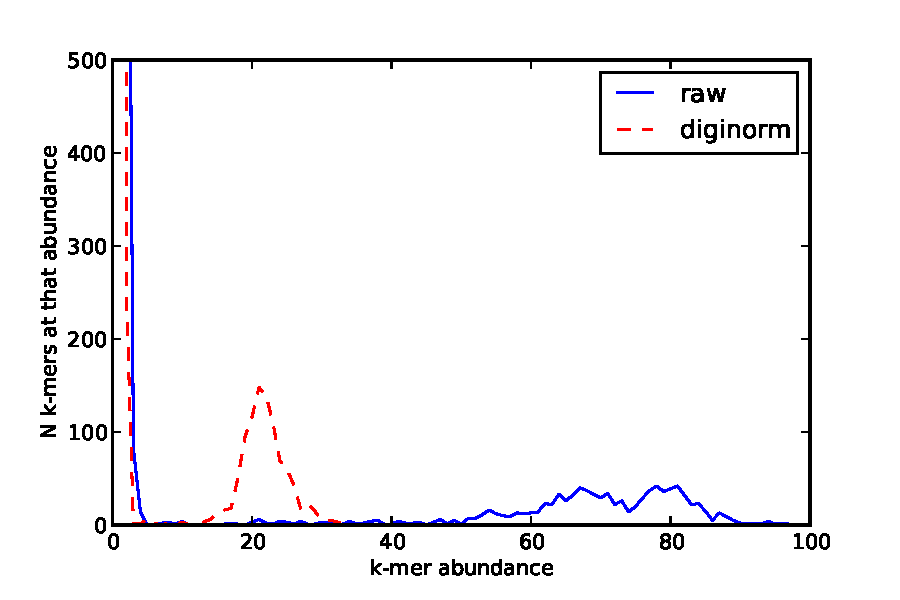
\includegraphics[width=4in]{./figures/kmer-spectrum}}
\caption{\bf K-mer spectrum of a simple artificial data set, before
  and after digital normalization.  The peaks at the origin represents
  erroneous k-mers resulting from (simulated) error; the peaks
  centered at 80 (original) and 20 (diginorm) represent k-mers truly
  present in the genome, which are shared among many reads.}
\label{fig:spectrum}
\end{figure}

% note, need to put in diginorm #s. Or do we? In Methods, maybe?

%% make compare2

\begin{table}

\centering
\begin{tabular}{|l|c|c|l|}
\hline
Name & Number of reads & Description \\
\hline
simple genome & 1000 & 1kb genome; no repeats \\
{\em E. coli} MG1655 & 4,863,836 & Subset of ERA000206 (\cite{chitsaz}) \\
simple transcriptome & 568 & 300:1 high:low abundance; shared exons \\
mouse mRNAseq & 7,915,339 & Subset of GSE29209 (\cite{trinityrna}) \\
simple metagenome & 2,347 & 316:1 high:low abundance species \\
mock metagenome & 18,805,251 & Subset of SRR606249 (\cite{podar}) \\
\hline
\end{tabular}

\caption{{\bf Data sets used for evaluation.}}

\label{tab:data}
\end{table}

We next used k-mer counts from the downsampled read set to detect
errors in the original read set.  The algorithm is straightforward: we
look for bases at the beginning or ends of low-abundance runs of
k-mers in each read, which should signify the locations of errors. We
used a ``trusted k-mer'' cutoff of $C_0 = 3$ as our abundance cutoff,
below which we assumed k-mers were erroneous (see Methods).  The
results are presented in Table~\ref{tab:a}.  Of the 633 simulated
reads from the simple genome that contain one or more errors, predicted
errors matched the known truth exactly for 485 of them (true
positives), and 366 reads were correctly predicted to contain no
errors (true negatives). 0 reads were falsely predicted to have no
errors (false negatives). The errors in 148 reads were miscalled --
while the reads each had one or more errors, the positions were not
correctly called -- and one read was incorrectly predicted to
contain errors, leading to a total of 149 false positives.  From this,
we calculated the prediction sensitivity to be 100\% and the
prediction specificity to be 71.1\%.

When we applied spectral error detection using the counts from the
original (un-normalized) reads, we saw similar results: 474 TP, 355
TN, 171 FP, and 0 FN, for a sensitivity of 100\% and a specificity of
67.5\% (Table~\ref{tab:a}).  (Note: for this analysis we used a cutoff
of $C_0=10$.)

%% make compare6 # original
%% make compare2 # dn

\begin{table}
\centering

\begin{tabular}{|l|c|c|}
\hline
{\bf Simple genome} & Original counts & Diginorm counts \\
\hline
Perfect detection (TP) & 474 & 485 \\
No errors (TN) & 355 & 366 \\
Miscalled errors (FP) & 159 & 148 \\
Mispredicted errors (FP) & 12 & 1 \\
Missed errors (FN) & 0 & 0 \\
\hline
Sensitivity & 100\% & 100\% \\
Specificity & 67.5\% & 71.1\% \\
\hline
\end{tabular}

\caption{{\bf Results from spectral error detection on 1000 synthetic
    reads from a simulated 10kb genome, using k-mer counts from
    original or digitally normalized reads.  The counts in the table
    are the number of reads where all errors were detected perfectly
    (TP), errors were present and none were called (TN), one or more
    errors were miscalled (one type of FP), errors were mistakenly
    called in an error-free read (the other type of FP), and errors
    present in a read were missed (FN).}}
\label{tab:a}
\end{table}

% make ecoli_compare2.txt

\paragraph{{\em E. coli} reads:}
We next applied digital normalization and k-mer spectral error
detection to an Illumina data set from {\em E. coli} MG1655
\cite{pubmed21926975}.  In real reads, we do not know the location of
errors; to calculate likely errors, we mapped 4.9m untrimmed reads to
the known {\em E. coli} MG1655 genome with bowtie2 \cite{bowtie2} and
recorded mismatches between the reads and the genome.  These
mismatches were taken to be errors in the reads.  We found 8.0m errors
in 2.2m reads, for an overall error rate of 1.60\%.

We then compared the results of k-mer spectral error detection with
and without digital normalization.  We used the same parameters as on
the simulated genome ($C_0=10$ for unnormalized, $C_0=3$ for
normalized).  The results are presented in
Table~\ref{tab:ecoli_dn_counts}. Using the original counts, the
sensitivities were close to the predictions from the normalized
counts: using the original counts, we achieved a sensitivity of
99.7\%, versus 99.2\% using the counts from the digitally normalized
reads.  The specificities were also comparable -- 68.8\% using the original
counts, and 68.7\% using the digitally normalized counts.

% make ecoli_compare2.txt
% make ecoli_compare2_nodn.txt

\begin{table}
\centering
\begin{tabular}{|l|c|c|}
\hline
{\bf E. coli} & Original counts & Diginorm counts \\
\hline
Distinct k-mers         & 39,677,503 & 26,510,104 (67\%) \\
\hline
Perfect detection (TP)  & 819,233   & 808,657 \\
No errors (TN)          & 2,782,265 & 2,782,403 \\
Miscalled errors (FP)   & 1,082,566 & 1,088,787 \\
Mispredicted errors (FP)& 177,637       & 177,499   \\
Missed errors (FN)      & 2,135     & 6,490    \\
\hline
Sensitivity & 99.7\% & 99.2\% \\
Specificity & 68.8\% & 68.7\% \\
\hline
\end{tabular}

% @CTB why FN so different??

\caption{{\bf Results from spectral error detection on 4.9m {\em
      E. coli} reads, using k-mer counts from original (left column)
    and digitally normalized (right column) reads.}}

\label{tab:ecoli_dn_counts}
\end{table}

\paragraph{{\em E. coli} error correction with Quake:}

% quake-ecoli-raw-cor.txt
% quake-ecoli-dn-cor.txt

\begin{table}
\centering
\begin{tabular}{|l|c|c|}
\hline
                                 & original    & diginorm \\
\hline
Total reads, after Quake         & 4,805,561   & 4,804,947 \\
Erroneous reads discarded        & 58,275      & 58,889 \\
Total bp                         & 441,752,819 & 441,701,309 \\
Total errors remaining           & 47,510      & 41,455 \\
Per-base error rate              & 0.011\%     & 0.009\% \\
\hline
\end{tabular}

\caption{{\bf Comparison of Quake results when run on the same {\em
      E. coli} data set, using k-mer counts from either the original
    data set (original) or the digitally normalized reads
    (diginorm).  All numbers are post-error correction; the original
    error rate was 1.60\%.}}

\label{tab:quake_ecoli}
\end{table}

% kmer-counts.txt

\begin{table}
\centering
\begin{tabular}{|l|c|c|c|c|}
\hline
Sample              & original unique k-mer count & normalized unique k-mer  count \\
\hline
{\em E. coli}       & 39,677,503 & 26,510,104 (67.8\%) \\
mouse mRNAseq       & 54,177,799 & 48,058,631 (88.7\%) \\
mock metagenome     & 201,459,416  & 201,093,236 (99.8\%) \\
\hline
\end{tabular}

\caption{{\bf Unique k-mer counts for original and normalized data
    sets using a k-mer size of 20 and the specified coverage cutoff.
    Digital normalization reduces the total number of k-mers in the
    data set for high coverage data sets.}}

\label{tab:kmer_counts}
\end{table}


% readstats.txt

\begin{table}
\centering
\begin{tabular}{|l|c|c|c|c|}
\hline
Sample              & original read count    &  normalized read count \\
\hline
{\em E. coli}       & 4,863,836   & 1,609,639 (33.1\%) \\
Mouse RNAseq        & 7,915,339   & 3,832,453 (48.4\%) \\
Mock metagenome     & 18,805,251  & 17,353,291 (92.2\%) \\

\hline
\end{tabular}

\caption{{\bf Read counts for original and normalized data sets using
    a k-mer size of 20 and the specified coverage cutoff. Digital
    normalization reduces the total number of reads for later analyses.}}
\label{tab:read_counts}
\end{table}

While the results above suggest that simple spectral error detection
works equally well both before and after digital normalization, we
were concerned that we might lose informative reads and k-mers during
digital normalization.  To evaluate this, we used Quake \cite{quake}
to perform error correction on the data set using the k-mer counts
from the digitally normalized reads, and compared the results to error
correction with the entire read data set.

The results of running Quake on the original data using counts from
the original and digitally normalized data are shown in
Table~\ref{tab:quake_ecoli}.  The performance was essentially the
same: Quake brought the overall error rate in the data set from 1.60\%
(8.0m errors) to 0.01\% (40,000 errors).

These results demonstrate that digitally normalized counts retain all
of the information necessary for effective error correction with
Quake, despite there being many fewer k-mers
(Table~\ref{tab:kmer_counts}) and far fewer reads
(Table~\ref{tab:read_counts}) being used as input into the k-mer count
table.

\subsection{Coverage-normalized data can be used to locate errors in variable
coverage shotgun sequencing data}

One of the drawbacks of spectral
abundance analysis is that it does not directly apply to data with
variable coverage.  For example, metagenomic or transcriptomic data
sets typically contain reads from both high-abundance and
low-abundance molecules.  This in turn leads to high coverage and low
coverage reads in the same data set. This variability in coverage
confounds naive spectral analysis for two reasons: first, erroneous
k-mers from very high abundance regions can accumulate and increase in
abundance over the threshold for trusted k-mers, thus appearing to be
correct (the so-called ``curse of deep sequencing'' \cite{Roberts2011}); and second, correct reads from low coverage regions yield
k-mers below the trusted k-mer threshold that appear to be incorrect.
In practice, therefore, error analysis for metagenomic and
transcriptome data uses other approaches than direct spectral error
analysis \cite{Medvedev2011, seecer, freclu}.

Digital normalization works on genomic data, with even coverage, as
well as on variable coverage data such as transcriptome and metagenome
data \cite{Brown2012, Lowe2015, Howe2014}.  Using the reference-free estimator
of per-read coverage developed for digital normalization, the median
k-mer abundance within a read, we developed a general approach that
enables spectral error analysis on variable coverage data.  We then
applied this to two synthetic data sets as well as two real data sets,
a mock shotgun metagenome and mRNAseq data from mouse.

\begin{figure}[!ht]
 \centerline{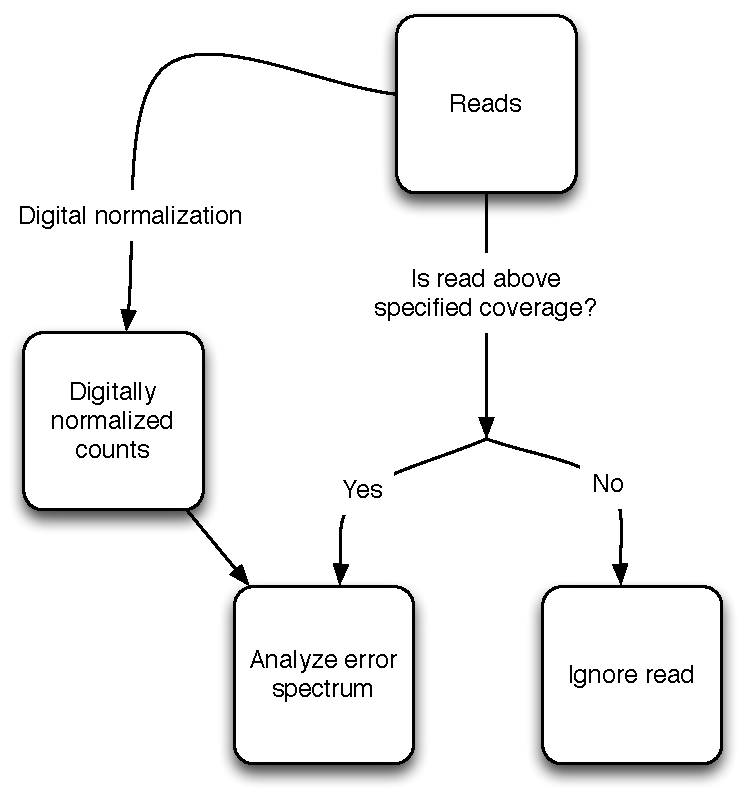
\includegraphics[width=3in]{./figures/coverage-aware-spectrum}}
\caption{{\bf Coverage-normalized spectral error analysis.  Reads are
    normalized, and high-coverage reads are subjected to spectral
    error analysis with the normalized counts, while low-coverage
    reads are ignored.}}
\label{fig:covaware}
\end{figure}

\paragraph{Coverage-normalized spectral error analysis:}

Using digital normalization, we should be able to address both the
problem of {\em too high} coverage and {\em too low} coverage.
First, by applying digital normalization to variable
coverage data and then working only with the k-mer counts from the
normalized reads, we can avoid counting high abundance errors as
correct.
Second, by ignoring reads with a low estimated coverage, we can
avoid misclassifying true low-abundance k-mers as errors.  The process
is shown in Figure~\ref{fig:covaware}.

% graph with read abundance spectrum, showing which reads we will
% call errors in?

\paragraph{Simulated data:}
To test this approach, we generated two more synthetic data sets,
``simple metagenome'' and ``simple mRNAseq,'' which contain both high-
and low-abundance species (see Table~\ref{tab:data} for data set
details).  After generating synthetic reads with a 1\% error rate and
applying digital normalization (k=20/C=20), we again used the normalized
counts to do spectral error detection.  However, we used a modified
algorithm that only examined reads with a median k-mer abundance of C
or greater.

% make rcompare2
% make mcompare2

\begin{table}
\begin{tabular}{|l|c|c|}
\hline
                            & {\bf simple mRNAseq } & {\bf simple metagenome}\\
\hline
Total reads                 & 568                   & 2347 \\
High coverage reads         & 524 (92.3\%)          & 2254 (96.0\%) \\
\hline
Perfect detection (TP)      & 228                   & 978 \\
No errors (TN)              & 235                   & 1098 \\
Miscalled errors (FP)       & 52                    & 170\\
Mispredicted errors (FP)    & 9                     & 6 \\
Missed errors (FN)          & 0                     & 2 \\
\hline
Sensitivity                 & 100\%                 & 99.8\% \\
Specificity                 & 79.4\%                & 86.2\% \\
\hline
\end{tabular}

\caption{{\bf Variable coverage spectral error detection on two synthetic
  data sets, a simple mRNAseq data set and a simple metagenome.
  Per-read coverage was estimated by median k-mer abundance within the
  read, and only the reads with estimated coverage at or above the
  specified threshold were analyzed.  Digitally normalized counts were
  used for the spectral error analysis.}}
\label{tab:spectra_variable}
\end{table}

The results of running error detection on the synthetic metagenome and
mRNAseq data sets are shown in Table~\ref{tab:spectra_variable}.

For the simple mRNAseq data
set, 524 of 568 reads (92.3\%) met the coverage criterion.  Of the
524 reads analyzed, the errors in 228 erroneous reads were called
perfectly (TP) and 235 of the reads with no errors were correctly
called as error-free (TN).  No reads were incorrectly determined
to be error-free (FN).  Of the remaining 61 errors, 52 were miscalled
(reads with errors were called correctly but the locations were
not correctly determined) and 9 reads were incorrectly called as erroneous
when they were in fact correct.  We calculated the prediction
sensitivity to be 100\% and the prediction specificity to be
79.4\%.
For the simple metagenome data set,
2254 of 2347 reads (96.0\%) met the coverage criterion, with 978 TP,
1098 TN, 2 FN, and 176 FP, for a prediction sensitivity of 99.8\% and
a prediction specificity of 86.2\%.  (In neither case did we include
low-coverage reads in the statistics.)

Importantly, these results are roughly comparable to the results on the
synthetic genome (100.0\% sensitivity and 71.1\% specificity with the
same parameters; see Table~\ref{tab:a}).

% make rseq_compare2
% make 

\begin{table}
\begin{tabular}{|l|c||c|}
\hline
& {\bf mouse mRNAseq} & {\bf mock metagenome} \\
\hline
Total reads                & 7,915,339          & 18,805,251       \\
High coverage reads        & 5,379,738 (68.0\%) & 4,954,341 (26.4\%) \\
\hline
Perfect detection (TP)     & 1,099,492          & 115,925          \\
No errors (TN)             & 3,560,733          & 4,723,053         \\
Miscalled errors (FP)      & 429,842            & 54,041           \\
Mispredicted errors (FP)   & 22,384             & 44,178          \\
Missed errors (FN)         & 267,287            & 17,144            \\
\hline
Sensitivity                & 80.4\%             & 87.1\%          \\
Specificity                & 88.7\%             & 98.0\%          \\
\hline
\end{tabular}

\caption{{\bf The results of variable coverage spectral error
    detection on two real variable coverage data sets, a mouse mRNAseq
    data set and a mock shotgun metagenome.  Per-read coverage was
    estimated by median k-mer abundance within the read, and only the
    reads with estimated coverage at or above the specified threshold
    were analyzed.  Digitally normalized counts were used for the
    spectral error analysis.}}
\label{tab:spectra_variable_real}

\end{table}

\paragraph{mRNAseq data:}

% rseq_compare2.txt

To evaluate coverage-normalized spectral analysis on real data, we
applied variable coverage spectral error analysis to 7.9m mouse mRNAseq
reads \cite{Haas2013}.  After calling errors in the reads by mapping
them back to the known genomes, we used spectral analysis to identify
putative errors.  The results are shown in
Table~\ref{tab:spectra_variable_real}, second column.  We achieved
80.4\% sensitivity and 88.7\% specificity on the 5.4m high coverage
reads in this data set.

\paragraph{Mock metagenome data:}

% podar_compare2.txt

We next applied our approach to 18.8m reads from a diverse mock community
data set \cite{podar}. We found 4,954,341 reads were at or above
this coverage threshold.  Here errors were again calculated by mapping
the reads to the known reference and finding mismatches.  The results
are shown in Table~\ref{tab:spectra_variable_real}, third column.  We
achieve 87.1\% sensitivity and 98.0\% specificity on the high coverage
reads.

\paragraph{Error correcting variable coverage data with Quake:}

% rseq_compare6.txt

There are many sophisticated error correction algorithms implemented
for shotgun genome data, but relatively few work directly on variable
coverage data such as mRNAseq \cite{Medvedev2011, seecer}.  Digital
normalization, in theory, could enable the use of {\em any} spectral
error correction algorithm on the high coverage components of data
sets.

To evaluate this, we again used Quake (a genomic error corrector) to correct
the high coverage mRNAseq reads using the diginorm counts.  We first
extracted the 5.4m reads with estimated coverage greater than or equal
to 20 from the mouse mRNAseq data set, and then digitally normalized
the data.  We next applied the Quake error corrector to the
unnormalized high-coverage reads using the k-mer counts from the
normalized reads, as with the {\em E. coli} data set.  Quake discarded
510,000 reads and corrected the remainder, bringing the error rate
from 1.0\% to 0.42\% - see Table~\ref{tab:quake_mrna}.  As with {\em
  E. coli}, this suggests that sufficient information remains in the
digitally normalized data to do an effective job of error correction.

% quake-ecoli-raw-cor.txt
% quake-ecoli-dn-cor.txt

\begin{table}
\centering
\begin{tabular}{|l|c|}
\hline
{\bf mRNAseq}                    & diginorm \\
\hline
Total reads                      & 7,915,339 \\
High coverage reads              & 5,379,738 \\
Erroneous reads discarded        & 509,979 \\
Total bp after correction        & 348,994,329 \\
Total errors remaining           & 1,469,618 \\
Per-base error rate              & 0.42\% \\
\hline
\end{tabular}

\caption{{\bf Results of running Quake on high-coverage reads from
    mouse mRNAseq, using k-mer counts from the digitally normalized reads.
    The original error rate was 1.0\%.}}

\label{tab:quake_mrna}
\end{table}

\subsection{A semi-streaming algorithm can be used for spectral error analysis}

The spectral error detection approach outlined above is a 2-pass
offline algorithm for any given data set - the first pass normalizes
the read set and records the k-mer abundances, while the second pass
analyzes the reads for low-abundance k-mers.  Even with digital
normalization reducing the number of k-mers under consideration, this
2-pass approach is time consuming on large data sets.  Below, we
develop an approach that considers many of the
reads only once (as in Figure~\ref{fig:summary}(b)).

\paragraph{Semi-streaming analysis of coverage-saturated regions:}

Shotgun sequencing oversamples most regions -- for example, for a 100x
coverage genomic data set, we would expect 50\% or more of the genome
to be represented by more than 100 reads.  This is a consequence of
the Poisson-random sampling that underlies shotgun sequencing
\cite{waterman}.  This oversampling provides an opportunity, however:
if we regard the read data set as a stream of incoming data randomly
sampled from a pool of molecules, high-abundance species or
subsequences within the pool will be more highly sampled in the stream
than others, and will thus generally appear earlier in the stream.
For example, in mRNAseq, highly expressed transcripts should almost
always be sampled much more frequently than low-expressed transcripts,
and so more reads from highly expressed transcripts will be seen in
any given subset.

With this in mind, we can adapt the same approaches used in previous
sections to do {\em semi-streaming} error analysis by detecting and
analyzing high-coverage reads {\em during} the first pass.  Here we
again use the median k-mer abundance of the k-mers in a read to
estimate that read's abundance \cite{Brown2012}; crucially, this can
be done at any point in a stream, by using the online k-mer counting
functionality of khmer to determine the abundance of k-mers seen thus
far in the stream \cite{Zhang2014}.

The conceptual idea is presented in Figure~\ref{fig:concept}.  On the
first pass, low-coverage reads would be incorporated into the k-mer
database and set aside for later analysis, while high-coverage reads
would be analyzed for errors. On the second pass, the set aside reads
would be checked for coverage again, and either ignored or analyzed
for errors.  Crucially, this second pass involves {\em at most}
another full pass across the data, but only when the entire data set
is below the coverage threshold; the larger the high coverage
component of the data, the smaller the fraction of the data that is
examined twice.

\begin{figure}[!ht]
\centerline{\includegraphics[width=4in]{./figures/graph-saturation}}
\caption{\bf Diagram of semi-streaming error detection. In a first pass
over the read data, reads are loaded in until the graph locus to which
they belong is saturated.  From that point on, reads are examined for
errors and not loaded into the graph.  In a second pass, only the subset
of reads loaded into the graph are examined for errors.}
\label{fig:concept}
\end{figure}

In Figure~\ref{fig:saturation}, we show diginorm-generated coverage
saturation curves for both real and error-free simulated reads from
{\em E. coli} MG1655.  In both cases, after the first 1m reads, the
majority of reads have an estimated coverage of 20 or higher, and
hence can be used for error analysis on the remainder of the data
encountered in the first pass.

% make compare4
% make mcompare4
% make rcompare4

\begin{table}
\centering
\begin{tabular}{|l|c||c||c|}
\hline
& {\bf simple genome}     & {\bf simple mRNAseq} & {\bf simple metagenome} \\
\hline
Number of passes & 1.32 & 1.16 & 1.33 \\
\hline
Perfect detection (TP)    & 485                 & 228     & 977 (-1) \\
No errors (TN)            & 365 (-1)            & 235     & 1095 (-3) \\
Miscalled errors (FP)     & 148                 & 52      & 171 (+1) \\
Mispredicted errors (FP)  & 2 (+1)              & 9       & 9 (+3) \\
Missed errors (FN)        & 0                   & 0       & 2 \\
\hline
Sensitivity               & 100.0\%             & 100.0\% & 99.8\% \\
Specificity               & 70.9\%              & 79.4\%  & 85.9\% \\
\hline
\end{tabular}
\caption{{\bf Results from applying semi-streaming error detection to the
    same synthetic data sets as in Table~\ref{tab:a} and
    Table~\ref{tab:spectra_variable}.  Number of passes is the average
    number of times each read in the data set was examined; numbers in
    parentheses give the difference between these numbers and the
    previous results.}}
\label{tab:spectra_streaming}

\end{table}

Moreover, because only the normalized counts are used in spectral
analysis, the approach should apply equally well to data sets with
uneven coverage, i.e. metagenomes and transcriptomes.  To test this,
we first apply this semi-streaming error detection approach to the three
synthetic data sets used earlier, and then to the three real data
sets.

\paragraph{Streaming error analysis of synthetic data:}

Using the semi-streaming approach on the ``simple genome'' reads, we obtain
nearly identical numbers to the full two-pass approach: 485 TP, 365
TN, 150 FP, and 0 FN, for a sensitivity of 100\% and a specificity of
70.9\% (Table~\ref{tab:spectra_streaming}).  However, with the
semi-streaming algorithm, only 320 of the 1000 reads are examined twice.
Likewise, for the ``simple mRNAseq'' and ``simple metagenome'' data
sets, we obtain identical and nearly identical results, respectively;
due to differences in the order in which reads are examined, the
simple metagenome fails to detect one true positive and erroneously
finds errors in three extra reads.  On the mRNAseq data set, 33.1\% of
the reads are examined twice, and on the metagenome, 380 of 2347
(16.2\%) of the reads are examined twice.

\paragraph{Semi-streaming error analysis of real data:}

% ecoli_compare4.txt

% rseq_compare4.txt

% podar_compare4.txt

\begin{table}
\begin{tabular}{|l|c||c||c|}
\hline
& {\bf \em E. coli} & {\bf mouse mRNAseq} & {\bf mock metagenome} \\
\hline
Number of passes         & 1.33      & 1.48         & 1.92 \\
\hline
Perfect detection (TP)   & 810,896   & 1,162,662 (+61,370 & 116,833  \\
No errors (TN)           & 2,781,961 & 3,552,261  & 4,717,494 \\
Miscalled errors (FP)    & 1,087,775 & 418,481    & 53,349 (-692)  \\
Mispredicted errors (FP) & 177,914   & 30,856 (+8472)    & 49,737 (+5559)  \\
Missed errors (FN)       & 5263 (-1227)     & 215,478 (-51,809)  & 16,928  \\
\hline
Sensitivity            & 99.4\%      & 84.4\% (+4.0\%)     & 87.3\%  \\
Specificity            & 68.7\%      & 88.8\%     & 97.9\%  \\
\hline
\end{tabular}
\caption{{\bf Results from applying semi-streaming error detection to the same
  real data sets as in Table~\ref{tab:ecoli_dn_counts} and
  Table~\ref{tab:spectra_variable_real}.  Number of passes is the average
  number of times each read in the data set was examined; unless noted in
  parentheses, numbers were within 1\% of non-streaming results.}}
\label{tab:spectra_streaming_real}

\end{table}

We also get similar quality results on the real data sets when
comparing two-pass error detection with semi-streaming error detection
(Table~\ref{tab:spectra_streaming_real}).  For {\em E. coli}, with
semi-streaming error detection we obtain a sensitivity of 99.4\% and a
specificity of 68.7\%, compared to 99.2\% and 68.7\% with the two-pass
approach (Table~\ref{tab:ecoli_dn_counts}).  For the mRNAseq data set,
we see a sensitivity of 84.4\% with semi-streaming vs 80.4\% with two-pass,
and a specificity of 88.8\% vs 88.7\% for semi-streaming vs two-pass,
respectively.  And for the mock metagenome, we have a sensitivity of
87.3\% with semi-streaming, vs 87.1\% with the two-pass approach; and a
specificity of 97.9\% for semi-streaming and 98.0\% two-pass (compare
Table~\ref{tab:spectra_streaming_real} and
Table~\ref{tab:spectra_variable_real}).  However, the semi-streaming
approach examined the {\em E. coli} data only 1.33 times, the mRNAseq
data 1.48 times, and the metagenome data 1.92 times on average.

\subsection{A semi-streaming algorithm can be used for error trimming}

Once errors can be {\em detected} with a semi-streaming algorithm, errors
can also be {\em removed} by trimming reads at the first base
predicted to be erroneous in a read.  This approach is remarkably
effective, but can require considerably more memory than quality-score
based trimming \cite{Zhang2014}.  Moreover, it is generally
implemented as an offline (two-pass) algorithm.  Below, we apply the same
semi-streaming approach shown in Figure~\ref{fig:concept} to trimming
reads.

%  (While it is possible to split reads around errors
%rather than truncating them, this introduces complications in
% downstream read processing.)

% make compare5

\paragraph{Semi-streaming error trimming on synthetic data:}

On the ``simple genome'' with counts from the digitally normalized
reads, this trimming approach eliminates 149 reads entirely and
truncates another 392 reads.  Of the 100,000 bp in the simulated
reads, 31,910 (31.9\%) were removed by the trimming process.  In
exchange, trimming eliminated {\em all} of the errors, bringing the
overall error rate from 0.63\% to 0.00\%.

% make mcompare5
% make rcompare5

For the simple metagenome we used the variable abundance approach
described above and only trimmed reads with estimated coverage of 20
or higher.  Here, of 2347 reads containing 234,700 bp, 314 reads
(13.4\%) were removed and 851 reads (36.3\%) were trimmed, discarding
a total of 74,321 bases (31.7\%).  Of 1451 errors total, all but 61
were eliminated, bringing the overall per-base error rate from 0.62\% to
0.04\%.  The simple mRNAseq data set showed similar improvement: 83 of
568 reads were removed, and 208 were trimmed, removing 19,507 of
56,800 bases (34.34\%).  The initial error rate was 0.65\% and the
final error rate was 0.07\%.
\paragraph{Semi-streaming error trimming on real data:}

% ecoli-report-untrim.txt ('make ecoli-report-untrim.txt')
%posfile ecoli-reads.sam.pos: 2177509 mutated reads of 4960248; 7990149 mutations total
%496024800 bp total
%overall error rate: 1.610837%

% ecoli-report-trim.txt ('make ecoli-report-trim.txt')
%posfile ecoli-abundtrim.sam.pos: 164655 mutated reads of 4861345; 203345 mutations total
%434621201 bp total
%overall error rate: 0.046787%

% output of 'make ecoli-mapped.fq.gz.abundtrim'
%
% read 4960248 reads, 496024800 bp
% wrote 4861345 reads, 434621201 bp
% removed 98903 reads and trimmed 2030456 reads
% trimmed or removed 12.38% of bases (61403599 total)
% fp rate estimated to be 0.004

Applying the semi-streaming error trimming to the {\em E. coli} MG1655 data
set, we trimmed 2.0m reads and removed 50,281
reads entirely.  Of 8.0m errors, all but 203,345 were removed,
bringing the error rate from 1.49\% to 0.07\%.  Trimming discarded 53
Mbp of the original 486 Mbp (11.1\%).

% rseq_compare5.txt
% rseq_compare5b.txt

% make podar_compare5

On the mouse mRNAseq data set, semi-streaming error trimming removed 919,327
reads and trimmed 648,322 reads, removing 19.8\% of the total bases,
bringing the overall error rate from 1.59\% to 1.21\%.  When we measured
only the error rate in the high-coverage reads, trimming brought the
error rate from 1.20\% to 0.42\%.  On the mock metagenome data set,
27,554 reads were removed and 171,705 reads were trimmed, removing 0.36\%
of bases; this low percentage is because of the very low coverage of
most of the reads in this data set.

\subsection{Illumina error rates and error profiles can be determined from a
small sample of sequencing data}

\begin{figure}[!ht]
 \centerline{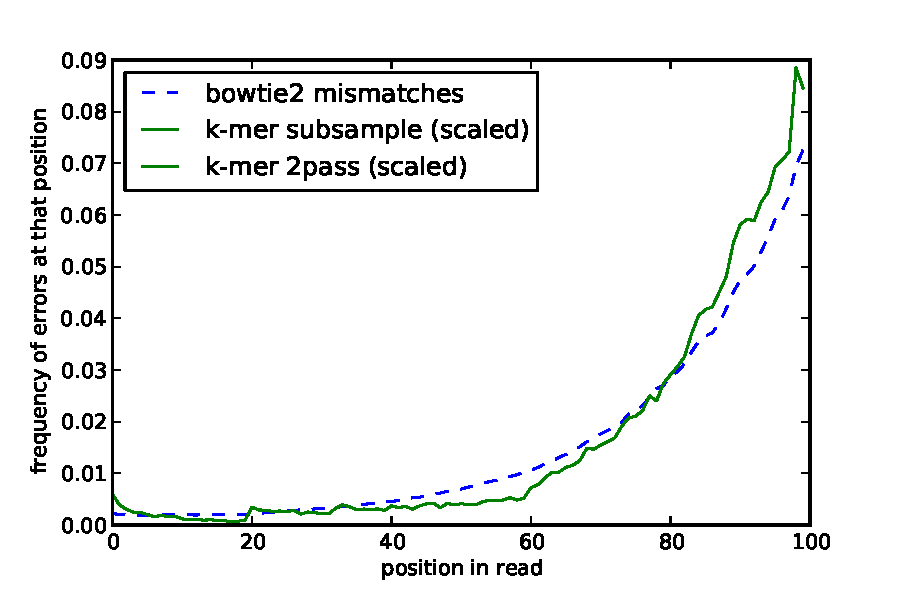
\includegraphics[width=4in]{./figures/ecoli-errhist}}
\caption{{\bf Error spectrum of reads in the {\em E. coli} data
    set. The sublinear k-mer spectrum analysis is calculated based on
    saturation of a fraction of the data set, while the two-pass
    spectral analysis uses all of the data.  bowtie2 mismatches are
    based on all mapped reads.  The y values for the k-mer spectral
    analyses are scaled by a factor of four for ease of comparison.}}
\label{fig:ecoli_err}
\end{figure}

\begin{figure}[!ht]
 \centerline{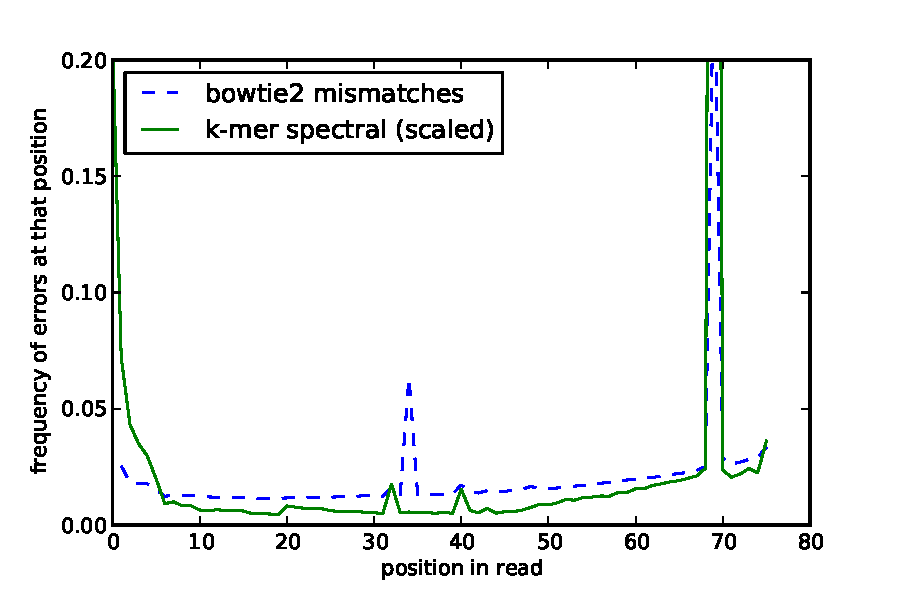
\includegraphics[width=4in]{./figures/rseq-errhist}}
\caption{{\bf Error spectrum of reads in the mouse RNAseq data set.
    The sublinear k-mer spectrum analysis is calculated based on
    saturation of a fraction of the data set, while the two-pass
    spectral analysis uses all of the data, and bowtie2 mismatches are
    based on all mapped reads.  The peak of errors at position 34 in
    the bowtie2 mapping reflects errors that in the first part of the
    data set are called as Ns, and hence are ignored by the sublinear
    error analysis; see text for details. Note, the bowtie2 mismatch
    rates are larger than the spectral rates, so for ease of
    comparison the y values for the k-mer spectral analyses are scaled
    by a factor of four.}}
\label{fig:rseq_err}
\end{figure}

With Illumina sequencing, average and per-position error rates may
vary between sequencing runs, but are typically systematic within a
run \cite{drisee}.  Melsted and Halldorson (2014) introduced an
efficient streaming approach to estimating per-run sequencing error,
but this approach does not apply to error rates by position within
reads \cite{Melsted2014}.  Here, k-mer spectral error analysis can be
used to calculate per-position relative sequencing error for entire
data sets \cite{Zhang2014}.

We can adapt the streaming approaches above to efficiently provide
estimates for {\em subsets} of the data.  The basic idea is to consume
reads until some reads have saturated, and then to calculate error
rates for new reads from the saturated loci in the graph.  This
can be done in one pass for data sets with sufficiently high coverage
data: as shown above (Figure~\ref{fig:saturation}), in some data sets,
most of the reads will have sufficient coverage to call errors by the
time 20\% of the data set has been consumed.

Using the same error detection code as above, we implemented a
sublinear memory/sublinear time algorithm that collects reads until
some regions have reached 20x coverage, or 200,000 reads have
surpassed a coverage of 10x (see Methods for details).  In either
case, all reads at or above a coverage of 10 are analyzed for errors,
with a trusted k-mer cutoff of 3.  In Figure~\ref{fig:ecoli_err} and
Figure~\ref{fig:rseq_err} we show the resulting error profiles for the
{\em E. coli} and mouse RNAseq data sets, compared with the profile
obtained by examining the locations of mismatches to the references.
We also show the error profile obtained with the full two-pass approach
(using digital normalization and then error detection as above)
for comparison.

In the {\em E. coli} data set (Figure~\ref{fig:ecoli_err}), we see the
increase in error rate towards the 3' end of the gene that is
characteristic of Illumina sequencing \cite{biases}.  All three error
profiles agree in shape (Pearson's correlation of 0.99 between each
pair) although they are offset considerably in absolute magnitude.
The k-mer error profile was calculated from the first 850,000 reads, but
is consistent across five other subsets of the data chosen randomly
with reservoir sampling (data not shown); all five subsets had
Pearson's correlation coefficients greater than 0.99 with the
bowtie2 mapping profile and the two-pass spectral approach.

The RNAseq error profile exhibits two large spikes, one at position 34
and one at position 69.  Both spikes appear to be genuine and
correlate with large numbers of Ns in those positions in the original
data set.  The spikes are present in the profiles derived from
two-pass spectral analysis as well as the bowtie2 mismatch
calculation.  However, the sublinear approach does not detect them
when using the first 675,000 reads.  This is because of the choice of
subsample: five other subsamples, chosen randomly from the entire data
set with reservoir sampling, match the match the two-pass spectral
analysis (data not shown).  The error profiles calculated from all six
subsamples with the sublinear algorithm have a Pearson's correlation
coefficient greater than 0.96 with the error profiles from the full
two-pass spectral approach and the bowtie2 mismatches.

% @CTB discuss subsample in discussion

\subsection{Performance on full mRNAseq and metagenomic data sets}

In practice, the space and time performance of both digital
normalization and the generalized streaming approach presented here
depend on specific details of the data set under analysis and the
precise implementation of the coverage estimator. While our intention
in this paper is to demonstrate the general streaming approach, we
note that even our naive implementation for e.g. streaming trimming is
useful and can be applied to very large data sets.  For high coverage
data, we can efficiently error-trim 10s of millions of reads in both
sublinear memory and fewer than two passes across the data.  In
Table~\ref{tab:full_trimming}, we show the summary statistics for
streaming error trimming of the full mouse mRNAseq and mock metagenome
data; in contrast to the smaller subsets used previously (see
Table~\ref{tab:trimming}), when we consider the full data sets the
majority of reads are examined only once (see ``Number of passes'',
Table~\ref{tab:full_trimming}).


% ecoli-report-untrim.txt, ecoli-report-trim.txt
% rseq_compare5.txt
% rseq_compare5b.txt
% podar_
% podar_compare5b

\begin{table}
\begin{tabular}{|l|c|c|c|c|}
\hline
Data set        & pre-trim error & \% bp trim & \% reads trim & post-trim error \\
\hline
{\em E. coli}   & 1.49\%         & 11.05\%          & 41.9\%      & 0.07\% \\
\hline
mouse mRNAseq   & 1.59\%         & 13.9\%           & 19.8\%      & 1.21\% \\
(high coverage only) & 1.20\%    & 20.4\%           & 29.0\%      & 0.42\% \\
\hline
Mock metagenome & 0.31\%         & 0.4\%            & 1.1\%       & 0.28\% \\
(high coverage only) & 0.16\%    & 1.4\%            & 3.5\%       & 0.07\% \\
\hline
\end{tabular}

\caption{{\bf A summary of trimming statistics for semi-streaming
    error trimming.  Error rates before and after trimming were
    estimated by mapping. ``High coverage'' numbers refer to the
    subset of reads with $C \geq 20$ that were subject to analysis.}}
\label{tab:trimming}
\end{table}



% cmouse-compare5-post.txt  cpodar-compare5-post.txt
% cmouse-compare5-pre.txt   cpodar-compare5-pre.txt

\begin{table}
\centering
\begin{tabular}{|l|c||c|}
\hline

Data set             & mouse mRNAseq      & mock metagenome \\
\hline
Total reads          & 81.3m         & 103.2m \\
Total bp             & 6.18 Gbp      & 10.4 Gbp \\
High-coverage reads  & 74.6m         & 91.9m \\
Number of passes     & 1.18          & 1.43 \\
\% reads trim        & 25.0\%        & 11.75\% \\
\% bp trim           & 13.74\%       & 4.03\% \\
Pre-trim error rate  & 1.89\%        & 0.27\% \\
Post-trim error rate & 1.30\%        & 0.15\% \\
\hline
\end{tabular}

\caption{{\bf Results of streaming error trimming on complete data sets.
Error rates before and after trimming were estimated by mapping.}}
\label{tab:full_trimming}
\end{table}

\section{Discussion}

\subsection{Digital normalization can be applied effectively to short reads prior to error detection and correction.}

Tracking k-mer abundances in large short-read data sets is part of
many error detection and correction algorithms, but this process can
be time and memory intensive.  Here we show that for some data sets
and several analyses, digital normalization can be used to reduce the
total number of k-mers under consideration without strongly affecting
results.

For example, with a real {\em E. coli} data set, digital normalization
reduced the number of k-mers by a third
(Table~\ref{tab:ecoli_dn_counts}, Distinct k-mers) while spectral
error prediction yielded essentially the same sensitivity and
specificity of error predictions (compare columns in
Table~\ref{tab:ecoli_dn_counts}).  Moreover, when we ran the Quake
error corrector on the reads using unnormalized and normalized counts
(Table~\ref{tab:quake_ecoli}), we achieved nearly identical results,
demonstrating that the digitally normalized data set retained all of the
information necessary for error correction.

\subsection{K-mer counts from digitally normalized reads can be used to error correct mRNAseq data}

Spectral error correction approaches typically rely on assumptions of
uniform sequence coverage, but these assumptions are violated by
several types of data, including mRNAseq and shotgun metagenome data.
Digital normalization can be used to generate k-mer spectra with even
coverage, allowing existing spectral error analysis approaches to be
applied to data from samples with non-uniform abundances.  We
demonstrated this by using spectral error detection with digitally
normalized data to predict errors in both synthetic and real RNAseq
and metagenome data (Tables~\ref{tab:spectra_variable} and
\ref{tab:spectra_variable_real}).  We then again used Quake to error
correct high-coverage portions of an mRNAseq data set, which yielded
promising results (Table~\ref{tab:quake_mrna}), although we note
that the unusually high per-position error rate in this data
may have led to poor results (Figure~\ref{fig:rseq_err}).

This again demonstrates that digitally normalized data retains the
information necessary to error correct high coverage reads, despite
having many fewer k-mers and total reads (Table~\ref{tab:kmer_counts}
and Table~\ref{tab:read_counts}).  Note that we used the Quake software
because it provided the option of using k-mer counts separate from the
reads under analysis.  While improved error correction algorithms
exist and could be evaluated with some modification, we believe the
best path forward is to integrate the semi-streaming approach into
an error corrector (below).

\subsection{Short-read error detection can be done efficiently with a streaming few-pass sublinear-memory algorithm}

K-mer spectral error detection, trimming, and correction approaches
are typically implemented as a two-pass offline algorithm, in which
k-mer counts are collected in a first pass and then reads are
corrected in a second pass.  While several algorithms that run in
sublinear memory do exist (e.g., Lighter \cite{lighter}), these are
still offline algorithms that require two or more passes across
the data.

In high coverage data sets it is possible to implement a more
algorithmically efficient approach, by detecting reads that are high
coverage in the context of reads previously encountered in the same
pass of the data.  We implemented this by integrating k-mer spectral
error analysis directly into the digital normalization algorithm, and
showed that on several synthetic and real data sets, we achieved
nearly identical predictions to the full two-pass algorithm with an
algorithm that is less than two pass (compare
Table~\ref{tab:spectra_variable_real} to
Table~\ref{tab:spectra_streaming_real}).

This near-equivalence of results is somewhat surprising, in that we
appear to be able to reduce a two-pass offline algorithm to a
semi-streaming approach requiring sublinear memory and fewer than two
passes with little alteration of results.  While data set
characteristics affect the algorithmic performance (see ``Time and
space considerations'', above), the algorithm performs {\em more
  efficiently} with {\em more} data -- a good trend.

As with digital normalization, a basic semi-streaming approach is very
simple to implement: with an online way to count k-mers, the algorithm
is approximately 10 lines of Python code.  The approach also requires
very few parameter choices: the only two parameters are k-mer size and
target coverage.  However, we do not yet know how these parameters
interact with read length, error rate, or data set coverage;
systematic evaluation of parameters and the development of underlying
theory is left for future work.  In practice, we expect that
additional work will need to be done to adapt existing error
correction approaches to use the semi-streaming approach.

\subsection{Error trimming can be done efficiently with a semi-streaming algorithm}

We next adapted the error detection algorithm to do semi-streaming
error trimming on genomic, metagenomic, and transcriptomic data.  On
high coverage components of variable coverage data sets, this led to a
substantial decrease in errors - up to an order of magnitude
(Table~\ref{tab:trimming}).

The implementation of semi-streaming error trimming used in this paper is
somewhat inefficient, and relies on redundantly storing all of the
reads needed for the second pass on disk during the first pass.  In
the worst case, where all reads are low coverage, a complete copy of
the data set may need to be stored on disk!  This is an area for
future improvement.  However, when we look at full data sets, fewer
than half the reads are examined twice (see Number of passes,
Table~\ref{tab:full_trimming}).

\subsection{Data-set wide error profiles can be calculated in sublinear time and memory}

The ability to analyze high-coverage reads without examining the
entire data set offers some intriguing possibilities.  One concrete
application that we demonstrate here is the use of high coverage reads
to infer data-set wide error characteristics for shotgun data, in a
way that is robust to the sample type \cite{drisee}.  This approach
could also be integrated directly into sequencers to assess whether
the target coverage has been obtained, and perhaps stop sequencing.
More generally, the approach of using saturating coverage to truncate
computational analysis may have application to streaming sequencing
technologies such as SMRT and Nanopore sequencing, where realtime
feedback between sequencing and sequence analysis could be useful
\cite{pacbio,nanopore}.

\subsection{Worst-case and best-case scenarios: when is error
trimming best applied?}

Here we introduce an approach to removing erroneous k-mers from large
sequencing data sets with a semi-streaming algorithm that can be used
on variable coverage data sets.  When should this be applied?

The general semi-streaming algorithm is most time-efficient on data sets
where much of the data is high coverage, because the second pass
across the data is limited to the set of reads that is low coverage on
the first pass (Figure~\ref{fig:concept}).  Even though the coverage
of the data sets may not be known in advance, the approach is robust
to low-coverage data: low-coverage reads can simply be ignored.

One particularly appealing aspect of the variable coverage error
trimming approach is that it does not need to be modified for
different data sets: the underlying algorithm can be applied equally
to genomic, mRNAseq, and metagenome data sets, although read lengths,
error rates, and data set coverage will affect the quality of results.
On high coverage genomic data sets, trimming can be made more
stringent by eliminating all low-abundance k-mers as erroneous, but
even if this is not done, the underlying approach is equally
efficient.

Digital normalization was developed primarily to decrease the memory
requirements for De Bruijn graph assembly by eliminating erroneous
k-mers; diginorm can reduce the memory requirements for Velvet by more
than an order of magnitude \cite{Brown2012}.  However, diginorm also
alters the coverage of the data set, which may affect the performance
of assemblers or other downstream analysis steps that rely on
coverage.  While semi-streaming error trimming removes at least as many
k-mers as digital normalization (and generally should remove many
more), k-mer based error trimming should have a much smaller and far
less biasing effect on data set coverage.  Moreover, trimming
eliminates fewer reads than digital normalization.  This may
make trimming a more palatable pre-filter for assembly than digital
normalization.

We caution against using variable coverage error trimming before
mapping-based abundance analyses such as transcript quantification,
ChIP-seq, or variant calling.  Variable coverage error trimming
preferentially retains low-abundance reads and eliminates portions of
high abundance reads, which may bias results.

\subsection{Conclusions}

We describe a time- and memory- efficient algorithmic approach to
k-mer spectral error detection and read trimming based on read-local
analysis of coverage.  This approach can be applied generically to
variable coverage data, including mRNAseq and shotgun metagenome
reads.  Moreover, the approach should be straightforward to integrate
into existing k-mer based spectral analyses, including error
correction and assembly pipelines.  Future applications could include
semi-streaming error correction, reference-free variant calling, and
reference-free analysis of streaming sequencing data.

% CTB sparse graph construction?

\bibliography{2014-streaming}

\end{document}
